\chapter{仿真、规则示范与真实训练数据}
\label{chap:data}

本章说明训练数据究竟怎样产生、什么可以交给模型、什么只能用于验收。这里的数据来自本机 HD1910 小鸭子仿真中的实际执行记录。既没有让大模型凭空编造动作答案，也没有把“发出踢球命令”自动当成“踢球成功”。全文中的采集数量与样本均取自已经冻结的正式数据集。

\section{仿真里的小鸭子与三个球}

场景由 \texttt{scene.py} 读取本地 Microduck 的 \texttt{scene\_ball.xml} 后生成。机器人有可移动、可转动的自由基座，躯干主体名为 \texttt{trunk\_base}。底层策略控制 14 个关节：每条腿各有髋偏航、髋侧摆、髋俯仰、膝、踝，共 10 个；颈俯仰及头部俯仰、偏航、侧摆，共 4 个。嘴部不在当前 14 维控制输出中，所以这轮技能训练并没有实现“张嘴叫两声”或“叼布”。

动力学使用 CPU MuJoCo；\texttt{load\_scene(...,"hd1910")} 加载本地 HD1910 参数文件 \texttt{1910\_m6.json}，通过 BAM 执行器模型把关节目标变成力矩。记录中的 \texttt{actuator=sts3215} 是这套模拟实现的模型名称，不能据此认定实体机器人的实际舵机型号。当前名义配置为 5\,ms 物理步长、4 个物理步的命令延迟，即 20\,ms；电压、压降和延迟固定，不进行这部分的域随机化。它也不是原先 GPU/Warp 训练环境的逐位复现。

红、黄、蓝三个球都能在物理世界中运动、碰撞；球半径为 0.035\,m，场景为灰色棋盘地面。主集合随机抽取距离 0.3--0.6\,m、方位覆盖一整圈的位置，球之间至少相隔 0.20\,m。这里先均匀采样半径、再均匀采样角度，并非在圆环面积上均匀采样。复位时机器人躯干初始高度 0.12\,m，关节置于已有策略的 HOME 姿态，先执行 2\,s 站立，再开始任务记录。

球的位置、相机和接触都由同一个物理场景产生；踢球效果不是播放一段角色动画，也不是直接修改球坐标来假装踢中。实际关节目标、接触力、球运动与身体倾斜都有轨迹记录。

\section{两台虚拟相机：看到什么、装在哪里}

两台相机均由本项目额外添加，固定在 \texttt{trunk\_base} 上，不随头部关节单独转动。坐标是相对躯干的安装位置：$+X$ 朝前、$+Y$ 朝左、$+Z$ 朝上，单位为米。它们不是离地高度，也不是世界坐标。

\begin{longtable}{P{2.0cm}P{4.0cm}P{2.4cm}P{6.1cm}}
\hline
名称 & 躯干相对位置 & 俯视角／竖直视场 & 用途\\
\hline
\endhead
\texttt{front} & $(0.14,0,0.16)$ & $45^\circ/85^\circ$ & 朝前下方观察，用于发现远一些的球及接近过程。\\
\texttt{near} & $(0.17,0,0.12)$ & $110^\circ/90^\circ$ & 朝下并向后观察脚边，用于球已经接近身体后的精细对齐；会看见机器人自身。\\
\hline
\end{longtable}

代码中的俯视角以水平方向为起点，因此 $90^\circ$ 是正下方，$110^\circ$ 是越过正下方再朝后 $20^\circ$。近场相机解决的是前置相机脚边盲区；它是当前实验的虚拟传感器配置。以后若实体只有一台相机，需要重新确定安装位姿或调整方案，不能把双相机训练结果直接当成单相机能力。

每次观察先冻结一份物理状态，再从该状态渲染两幅 $320\times240$ 的 RGB，以及各自对齐的深度图。RGB 是 \texttt{uint8} 三通道图像；深度是以米为单位的光轴方向距离，保存为浮点数组。深度不是普通 RGB 的第四个颜色通道。仿真深度没有在这轮采集中加入真实深度相机的空洞和噪声。

\begin{figure}[htbp]
\centering
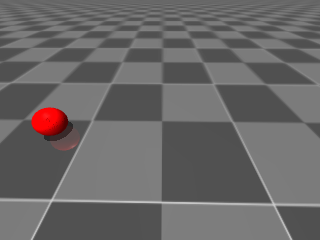
\includegraphics[width=.47\linewidth]{assets/sample_front.png}\hfill
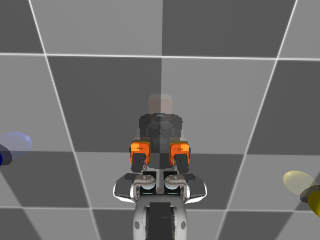
\includegraphics[width=.47\linewidth]{assets/sample_near.png}
\caption{真实训练首样本的 front（左）与 near（右），seed=1000，同一时刻。原指令为“现在能看到什么？”。这是机器人实际输入视角，未使用外部观察相机。}
\end{figure}

交互窗口左边的第三人称画面方便人观察机器人，右边显示 front 和 near。第三人称画面不送给 VLM，也不进入这次训练样本。训练实际输入的是两幅 RGB，另附 RGB-D 检测所得的结构化测量，而不是把整张深度图送进 Qwen 图像编码器。旧的 \texttt{dataset.py} 还保留过 RGB-only 导出接口；本轮正式数据使用新的 \texttt{training\_data.py}，不能用旧文件的简介推断当前输入。

\subsection{球的三维位置从哪里来}

\texttt{perception.py} 先按 RGB 通道阈值分别找红、黄、蓝区域，取至少 10 个像素的连通区域，再把像素和对应深度反投影成点云。它用已知球半径 0.035\,m 拟合球面，并检查曲率、内点比例、残差和可见球面的几何跨度，避免把一块同色地板误当成球。拟合中心通过相机安装旋转和平移变换到躯干坐标系。

检测记录包含颜色、球心 \texttt{center\_body\_m}、像素中心 \texttt{pixel\_uv}、拟合内点数 \texttt{pixels}、拟合残差 \texttt{fit\_residual\_m}、来源相机和 \texttt{confidence}。最后一个值是几何质量分数，并不是“有 90\% 概率正确”这样的校准概率。两台相机同时检测到同色球时，保留质量较高的一项；当前任务假设每种颜色只有一个球。

这条测量链没有读取球的世界坐标或物体分割 ID。不过它依赖颜色、球体形状和已知半径的先验，不能被称作“任意物体的通用识别”。身体的 yaw、倾角和静止判断则来自仿真状态，作为本体传感器的代理；迁移到实机时，需要相应的姿态和速度估计。应明确区分“没有把球的真值位置交给模型”和“输入完全没有仿真状态”。

本节核对：\texttt{scene.py}:10--75；\texttt{runtime.py}:23--44、51--119、281--334；\texttt{perception.py}:89--183。

\section{规则老师怎样选下一步}

采集时使用 \texttt{RuleVLMBackend} 处理语言与视野描述，再由 \texttt{KickPlanner} 处理踢球。虽然类名包含 VLM，它是一个规则接口实现，没有预训练神经网络参与这些示范。它根据本次 RGB-D 测量、机身状态和自身少量记忆，一次选择一个短动作；实际执行后重新看图，再决策。

下面给出真实优先级。前面的条件成立后就立即返回动作，因此不是把所有条件同时执行。

\begin{longtable}{P{2.2cm}P{8.0cm}P{4.4cm}}
\hline
阶段 & 真实判断 & 返回动作\\
\hline
\endhead
搜索 & 当前没有目标颜色。只在搜索期间累计包裹处理后的 yaw 变化，计算已覆盖角度范围。覆盖达到 $2\pi+0.25$\,rad 后仍不可见，则结束为未找到。 & \texttt{turn\_left}，1.0\,s；发现目标后清空搜索角度记录。\\
转向目标 & 球距躯干平面距离 $>0.24$\,m，或者球的 $x<0.03$\,m，且方位角绝对值 $>0.35$\,rad。 & 按角度符号左转或右转，0.6\,s。\\
选择并锁脚 & 首次满足目标 $x<0.24$\,m 时，$y\geq0$ 锁定左脚，否则锁定右脚。 & 保存内部脚别；后续使用该脚对应目标点。\\
站稳与踢球 & 球心与脚目标点的 $x,y$ 误差分别不超过 0.012\,m。首次对齐或身体未静止时先等待。 & 真正的对齐站立 0.6\,s；再次确认后踢对应脚 0.5\,s。\\
避开干扰球 & 还需前进，另一色球位于前方且 $x<\min(x_{\rm target},0.24)$、$|y|<0.10$\,m。 & 向该干扰球的反侧平移 0.32\,s。\\
横向对齐 & 远处 $x>0.24$\,m 时横向容差 0.05\,m，近处为 0.012\,m。 & 按横向误差正负左移或右移。\\
前后对齐 & 横向已满足容差，纵向误差仍大于 0.012\,m。 & 前进；若越过目标点则后退。\\
\hline
\end{longtable}

两只脚的标定目标球心分别是左脚 $(0.0895,0.0411)$\,m、右脚 $(0.0881,-0.0429)$\,m。横移时，$|dy|>0.07$ 用 0.32\,s，$|dy|>0.028$ 用 0.20\,s，更小误差向左用 0.06\,s、向右用 0.10\,s。前进时，$dx>0.12$ 用 0.60\,s，$dx>0.045$ 用 0.32\,s，其余用 0.26\,s；后退时，$dx<-0.04$ 用 0.32\,s，否则用 0.20\,s。这些不对称短脉冲是当前控制器下的工程参数，不是普适规律。

身体“静止”要求平面速度范数小于 0.025\,m/s、陀螺角速度范数小于 0.3\,rad/s。规则最多允许 120 次决策、180\,s 仿真任务时间；达到任一限制就失败退出。因此“转一圈找球”是有观测、有角度记录、有终止条件的搜索，不是简单播放固定时长后宣称已经搜遍。

每次非站立动作后，执行器自动站立恢复 1\,s；踢球后恢复 3\,s。规则自主选择的 0.6\,s 站立与上述固定恢复不同：前者表达“已经对齐，还要确认站稳”，应成为学习目标；后者属于执行协议，不应被重复学成上层决策。

本节核对：\texttt{planner.py}:14--97；\texttt{tasks.py}:114--159；\texttt{runtime.py}:293--295。

\section{676 个采集案例怎样组成}

采集计划在运行前固定，失败保留原分母，不因失败换 seed 重抽。一个 case 对应一个独立 episode，但一个 episode 可以含多个语言任务；一个任务又可产生很多次看图决策。三种数量不能混为一谈。

\begin{longtable}{P{3.0cm}P{5.8cm}P{5.8cm}}
\hline
集合 & 计划与独立 seed & 实际结果及目的\\
\hline
\endhead
随机主集合 & 100 seeds；每个 seed 三个颜色踢球 case，加一个连续对话 case，共 400。 & 随机踢球 277/300 通过；连续对话 100/100 通过。覆盖搜索、绕开干扰球、接近、对齐和问答。\\
近场左右脚补充 & 30 seeds；每个 seed 两只脚乘三种颜色，共 180。目标球在脚目标点周围各轴扰动 $\pm0.004$\,m。 & 180/180 通过，左右脚各 90。其他球距离 0.35--0.60\,m，用于补充稀少的踢球标签。\\
独立复位方向补充 & 16 seeds；每个 seed 前后左右移动及左右转六条指令，各自复位，共 96。 & 96/96 通过。同一 seed 六种指令的初始双图与状态完全相同，使动作必须随语言改变。\\
\hline
\end{longtable}

主集合的踢球 episode 按“描述当前视野、踢指定球、再次描述视野”运行。连续对话 episode 有 10 条任务：一次描述、六个方向动作、停止、再次描述、含糊踢球请求。语言包含换说法和否定干扰，如“别踢黄球，踢红球”。训练、验证、测试的命令模板分开，检验的不只是完全重复句子的记忆。

共计 146 个 seed，按组固定为训练 110、验证 18、测试 18。主集合分别是 1000--1079、1080--1089、1090--1099；近场集合是 2000--2019、2020--2024、2025--2029；独立方向集合是 3000--3009、3010--3012、3013--3015。同一 seed 的不同颜色和说法全部留在同一个 split，避免相似场景在训练和考试两边出现。

\subsection{成功和失败怎样确认}

踢球验收独立读取物理真值：要求指定脚在踢球开始后 0.54\,s 的窗口内碰到指定球，目标水平位移至少 0.12\,m，无机器人碰其他色球、无踢前提前碰目标球；全过程倾角小于 $30^\circ$、躯干不低于 0.065\,m。最后还须站立，倾角小于 $10^\circ$、平面速度小于 0.025\,m/s、角速度小于 0.3\,rad/s、躯干高度大于 0.09\,m。程序还检查轨迹和数值有效性。

这些结果是“规则老师在这批仿真里的验收结果”，不是预训练或微调 VLM 的成功率。近场任务已经把目标放在脚边，也不能与随机远近、可能需要转身寻找的任务混在一起报告一个令人误解的成功率。

23 个随机踢球失败任务中，9 个是验收未通过、12 个搜索未找到、2 个超时。原始图像、动作与失败原因全部保留；正式 SFT 排除这 23 个任务的全部动作和结束标签。不过它们所在 episode 各有两次独立成功的视野问答，这 46 个问答任务仍可保留。直接动作另检查身体稳定、无球接触以及实际位移／偏航方向，不能只检查文字解析正确。

\section{原始记录的文件和字段}

\begin{longtable}{P{4.0cm}P{10.6cm}}
\hline
文件 & 内容与用途\\
\hline
\endhead
\texttt{episode.json} & episode 身份、seed、后端、相机标定、初始布局、物理参数、软件版本、源码与三份 ONNX 哈希；采集补充 split、场景类型和独立验收状态。\\
\texttt{events.jsonl} & 每行一个事件，记录指令、观测、阶段、提议动作、真实执行时间、任务状态及回复。它是训练追溯的主索引。\\
\texttt{frames/*.png} & 每个观察时刻的 front／near RGB。\\
\texttt{frames/*\_depth.npz} & 同时刻深度，数组键为 \texttt{depth\_m}。\\
\texttt{trajectory.npz} & 时间、\texttt{qpos/qvel}、技能名、倾角、yaw、球与躯干位置、14 维网络原始动作、关节目标。供物理验收和回放。\\
\texttt{contacts.json} & 接触时间、技能、球颜色、另一球颜色、接触几何体名称及法向力。用于分辨真踢中、提前碰球和误碰。\\
\texttt{summary.json} & 每个语言任务的最终结果、独立验收指标、异常、仿真时长及墙钟时长。\\
\texttt{scene.xml}、日志 & 本次生成场景及初始化输出，帮助复现。\\
\hline
\end{longtable}

\begin{longtable}{P{3.4cm}P{11.2cm}}
\hline
事件字段 & 精确含义\\
\hline
\endhead
\texttt{event\_id}/\allowbreak\texttt{task\_id} & 分别定位一次事件和一个语言任务；不是模型应该据以猜动作的特征。\\
\texttt{instruction} & 用户本次原话；保留不同说法，不能替换成规则解析后的答案。\\
\texttt{intent/context} & 原始规则语义解析、历史选择等。只能按白名单重建学生输入，不能整包照搬。\\
\texttt{observation} & \texttt{frame\_id}、绝对仿真 \texttt{time\_s}、双图／深度相对路径、检测结果、yaw、静止状态与倾角。\\
\texttt{phase/decision} & 老师当前阶段和技能、时长、颜色；阶段属于审计信息，动作可成为目标标签。\\
\texttt{execution} & \texttt{started/completed} 明确是否真的开始、完成，另有开始／结束时间。提议本身不证明执行。\\
\texttt{done}/\allowbreak\texttt{status}/\allowbreak\texttt{reply} & 是否任务终结、成功／失败／澄清状态及回复。非动作事件允许没有 decision。\\
\hline
\end{longtable}

模型运行的日志还会有 \texttt{controller\_source} 和 \texttt{model\_trace}，保存原始回复、延迟、输入白名单、guard 结果等。本轮只接受规则示范来源，不会把模型自己的未验证预测悄悄回灌成正确答案。

\section{从原始轨迹到 11,934 条监督样本}

\texttt{training\_data.py} 逐任务检查完整结束事件、真实执行、时长一致、恢复配对、独立验收及部署 guard。验证通过后，留下每次真正需要模型选择的动作，再加一条结束、问答或澄清响应。9,063 条固定恢复事件不作为上层标签；100 条操作员停止任务也不经过模型学习，因为停止有即时独立通道。

最终共有 2,413 个合格任务、11,934 条决策样本：训练 9,500，验证 1,299，测试 1,135。导出复制了 23,868 张 RGB，每张与原记录 SHA256 一致；三个 split 都有九种技能和三种颜色。正式目录里的 \texttt{manifest.json} 保存哈希、接受／排除清单和统计；它是导出时的静态证明，当前训练是否运行应看训练目录的状态文件。

\subsection{真实样本：一次左脚踢红球}

以下来自正式 \texttt{train.jsonl} 第 8783 行，seed=2000，episode 后缀为 \texttt{160616\_a3617b51}，事件 \texttt{event\_00005}。完整未删节记录另存为本报告目录的 \texttt{sample\_kick\_original.json}。下方数值为便于阅读保留六位小数；这只是排版，训练文件保留原值。

\begin{figure}[H]
\centering
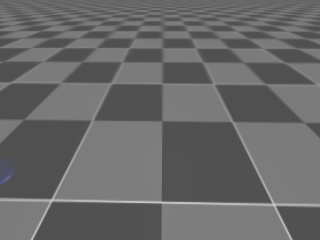
\includegraphics[width=.47\linewidth]{assets/sample_kick_front.png}\hfill
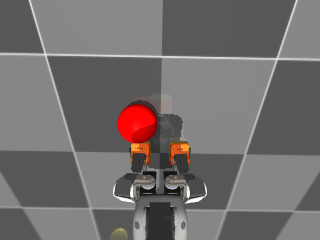
\includegraphics[width=.47\linewidth]{assets/sample_kick_near.png}
\caption{同一真实踢球样本：front 中目标红球不在视野；near 能看到脚边红球和机器人身体。前相机看不到目标，不等于两台相机都看不到。}
\end{figure}

\begin{Verbatim}[breaklines=true,fontsize=\small]
instruction = "踢红球"
state = {
  "yaw": 0.017050, "stationary": true,
  "tilt_deg": 1.392739, "sim_time_s": 0.6,
  "detections_rgbd": [{
    "color": "red", "camera": "near",
    "center_body_m": [0.090468, 0.039138, -0.080457],
    "pixel_uv": [138.0, 125.0], "pixels": 1231,
    "confidence": 0.806886, "fit_residual_m": 0.000196
  }]
}
context.previous_action = {
  "type":"skill","skill":"stand","seconds":0.6,
  "target_color":"red","reply":"保持站立，等待身体稳定。"
}
context.step = 1
context.selected_color = "red"
target = {
  "type":"skill","skill":"kick_left","seconds":0.5,
  "target_color":"red","reply":"执行左脚踢球动作。"
}
\end{Verbatim}

这份展示中的赋值写法用于讲解字段，不是可直接作为一行训练 JSON 的替代文件。context 还保存原样的 \texttt{previous\_feedback} 与一条 history：确认刚才的 stand 已执行，说明踢球任务应按新画面继续判断，执行过动作不代表踢球成功。history 的 action 与 previous\_action 相同，feedback 与 previous\_feedback 相同。以后较长任务最多保留最近六条。

这里 $z$ 为负，表示球心在躯干原点下方，并非无效深度。球心 $x,y$ 到左脚目标点的误差约为 $0.000968$\,m、$-0.001962$\,m，都小于 0.012\,m；机身也已静止。因此老师标注左脚踢 0.5\,s。该标签是规则示范，不能描述为“微调模型已经正确预测”。

原始事件观测时间约为 2.6\,s，任务首帧约为 2.0\,s，故 v5 输入时间为 0.6\,s。执行记录确认这次动作从约 2.6\,s 到 3.1\,s 完成；随后固定恢复 3\,s，再结束任务。训练只保留 stand0.6、kick0.5、finish 三次选择，恢复不是第四个需要预测的技能。

\subsection{逐字段变成模型消息}

导出行的 \texttt{images} 是数据集内双图相对路径；\texttt{instruction/state/context} 是真正输入；\texttt{target}、\texttt{label} 和 assistant 消息是同一个五字段目标。顶层 sample、episode、task、seed 及 \texttt{source} 保存追溯关系，不进入 user 文本。source 中的规则 phase、规则任务种类和真实执行时间也不是学生特征。

消息顺序固定为 system、user、assistant。system 是完整 v5 提示词；user 内容依次为“Current camera: front”、前图、“Current camera: near”、近图，最后一段 JSON 文本装入原指令、状态和历史。assistant 才放正确动作 JSON。训练器从 raw 字段重新构造同一结构，读取两张 PNG 为 RGB，交给 Qwen processor；processor 用 chat template 加上角色标记、图像占位和视觉张量。它不是只读取图片文件名就能看图。

构造 prompt 时只有 system 与 user，再加 assistant 开始标记；构造训练全文时才追加 target。程序核对前缀边界，不静默截断过长样本。模型需要预测 assistant 部分的 token，不能把 target、成功指标、未来图像混进 user，详细损失和张量处理见训练章节。

首条真实问答样本的指令是“现在能看到什么？”，老师回复“我现在看到左前方有红球，右后方有黄球。”其类型为 answer、skill 为 null、seconds 为 0。这里“视野”包括 near，所以右后方黄球可以被描述；回复没有因为场景配置固定有三球就声称看见蓝球。它证明数据里有视觉问答目标，不证明模型已具备开放世界对话能力。

\section{防止偷看答案，以及这批数据的边界}

v5 删除了模型 context 中的 \texttt{task\_id}，将绝对 episode 时间改为任务内相对秒数并舍入到微秒。原因是原连续指令顺序固定：如果“第二个任务总是前进”，模型可能根据任务编号或绝对时间猜答案。原日志仍保留编号与绝对时间方便排查；训练和部署共享同一过滤与时间函数。独立复位的六方向补充进一步提供“相同画面、不同语言、不同动作”的样本。

当前目标颜色来自原始指令；第一次决策不会得到规则已经解析好的当前 intent。执行过含颜色的动作后，历史中的 \texttt{selected\_color} 才可用于连续任务。真值只在旁路评价成功与否、筛选任务，不作为模型球心，也不会强迫模型在 finish 中声称已经成功。踢球结束标签使用“已执行踢球动作并恢复站立；是否踢中目标需要独立验收。”

\begin{longtable}{P{4.0cm}r r r}
\hline
技能标签 & 训练 & 验证 & 测试\\
\hline
\endhead
\texttt{stand} &342&60&56\\
\texttt{move\_forward} &1425&188&165\\
\texttt{move\_backward} &130&26&21\\
\texttt{move\_left} &2015&250&196\\
\texttt{move\_right} &2310&254&217\\
\texttt{turn\_left} &649&114&91\\
\texttt{turn\_right} &445&61&49\\
\texttt{kick\_left} &96&17&18\\
\texttt{kick\_right} &246&42&38\\
\hline
\end{longtable}

动作分布不均衡，横向调整明显多于后退与左踢；相邻样本也很相似，11,934 行不等于 11,934 个独立场景。随机完整踢球与已就位近场踢球必须分别评估，还要看每类技能及整任务完成情况。

老师有一个尚未完全显式化的记忆：第一次进入近区时锁定的脚别。六条动作历史不一定能恢复很久以前的决定，因而个别标签可能依赖学生未充分观测的状态。本轮已记录这一限制，没有把老师内部脚别偷偷塞给学生。以后可设计模型自己提交并保持的脚别记忆，再同步更改采集、训练和部署协议。

失败轨迹可用于诊断和以后构建纠错数据，但本轮并没有 DPO、chosen/rejected 配对或失败负样本损失。这轮 SFT 的目标是模仿经过筛选的正确技能选择，不是在训练过程中通过试错自动学会所有失败恢复。

本章数据证据：三个采集根目录的 \texttt{summary.json}、正式数据 \texttt{manifest.json}，以及独立审计 \texttt{training\_audit\_20261114/final\_dataset.json}；完整路径与关键行号列于 \texttt{sources\_local\_data.json}。
